\section{Separation von Amplitude und Phase}
\label{complex:separate}
\rhead{Separation Amplitude / Phase}

Bei den bisherigen Beispielen mit dem Haar- und Gabor-Wavelet haben wir gesehen, dass die Wahl des Wavelets das erhaltene Bild stark beeinflusst.
Beiden Beispielen gemein war jedoch, dass die Schwingung des Signals in der Amplitude erhalten blieb.
Das Skalarprodukt zwischen Signal und Wavelet ist also abhängig von der Phase maximal, null, minimal, null, maximal, \textellipsis

Diese Oszillation in der Amplitude ist unschön, da sich etwa $a_\text{max}(b)$ so nicht richtig bestimmen lässt.
Dieser Abschnitt dreht sich um die Lösung dieses Problems.
Ziel ist es, am Ende einen Operator $\Ana\,$ zu haben, der ein bestehendes Wavelet durch möglichst kleine Änderungen so anpasst, dass die Separation von Amplitude und Phase möglich wird.
Dazu gehen wir wie folgt vor.

Als erstes identifizieren wir negative Frequenzen als Ursache des Problems und zeigen, dass es kein reelles Wavelet geben kann, bei dem sich Amplitude und Phase einer Schwingung separieren lassen.

Daraus entwickeln wir einen Proototyp des Operators $\Ana\,$, und testen, ob er angewandt auf das Gabor-Wavelet, das gewünschte Resultat erzielt.

Ein kleiner Exkurs in die Signaltheorie erlaubt uns, den Operator $\Ana\,$ korrekt zu definieren. 
Dazu werden wir den Begriff des \emph{analytischen Wavelets} einführen.



Dann untersuchen wir, was das für das Wavelet bedeutet und versuchen diesen Operator zu bestimmen.

\subsection{Das Problem negativer Frequenzen}
Negative Frequenzen sind erstmal etwas unintuitiv.
Durch die Symmetrien
\[
	\cos(\omega t) = \cos(-\omega t)
	\quad
	\sin(\omega t) = -\sin(-\omega t)
\]
machen negative Frequenzen für reelle Signale auch nicht wirklich Sinn.
Die komplexe Exponential\-funktion kennt dieses Problem nicht.
Vielmehr gilt
\begin{equation}
	e^{i\omega t} = \overline{e^{-i\omega t}}.\label{complex:exp-inv-conj}
\end{equation}
Deshalb haben wir im Abschnitt~\ref{subsection:real-fourier-series} auch nur positive Frequenzen betrachtet,
bei den komplexen Fourierreihen im Abschnitt~\ref{subsection:complex-fourier-series} jedoch auch negative.

Cosinus und Sinus liefern -- in Analogie zu einem Kreis -- kartesische Koordinaten. 
Sie sind auch gleich Real- und Imaginärteil der komplexen Exponentialfunktion.
\[
\Re e^{i\omega t} = \cos(\omega t), \quad \Im e^{i\omega t} = \sin(\omega t)
\]
Für eine Darstellung als Betrag und Winkel benötigt man folglich immer beide koordinaten.
Der komplexe Raum bietet hingegen genug Platz, um beide Informationen zugleich darzustellen.
Die Exponentialfunktion
\[
	z(t) = Ce^{i\omega t} = |C|e^{i(\omega t + \arg C)}
\]
erlaubt durch 
\[
	|z(t)| = |C| 
	\quad \text{und}\quad
	\arg z = \arg \omega t + \arg C
\]
eine separate Betrachtung von Amplitude und Phase.


Komplexe Basisfunktionen alleine garantieren die Separierbarkeit von Betrag und Winkel jedoch noch nicht.
Diese beiden Teile müssen linear unabhängig sein.
Sind sie es nicht, so gilt
\[\Im \psi = \lambda \Re \psi, \quad \lambda \in \mathbb C.\]
und es folgt
\begin{align*}
	\psi &= \Re \psi + \Im \psi\\
	&= \Re \psi + \lambda \Re \psi\\
	&= (1+\lambda) \Re \psi.
\end{align*}
Hierbei ist $1+\lambda$ ein konstanter Faktor. 
Er kann aus der Wavelettransformation ausgeklammert werden und es folgt
\begin{align*}
	\Wave_\psi f 
	&= \langle f, \psi \rangle \\
	&= \langle f, (1+\lambda) \Re \psi \rangle \\
	&= \overline{1+\lambda} \langle f, \Re \psi \rangle \\
	&= (1+\overline{\lambda}) \Wave_{\Re\psi}f
\end{align*}
Ein solches Wavelet bringt also keinen zusätzlichen Nutzen gegenüber reellen Wavelets.
Wie aber finden wir zu einem gegebenen, reellen Wavelet einen passenden, orthogonalen Imaginärteil?

Betrachten wir wieder die Exponentialfunktion.
Bei ihr sind Real- und Imaginärteil orthogonal wie gewünscht.
Gewisse Kombinationen von komplexen Exponentialfunktionen führen jedoch wieder zu rein reellen Funktionen.
Dies gilt es zu vermeiden.

Mit Hilfe der komplexen Konjugation können Real- und Imaginärteil aber auch dargestellt werden als
\[
\Re \psi = \frac{\psi + \overline\psi}{2} 
,\quad
\Im \psi = \frac{\psi - \overline\psi}{2i}.
\]
Wenden wir dies auf die Exponentialfunktion an, so erhalten wir
\begin{equation}
	\frac{e^{i\omega t} + \overline{e^{i\omega t}}}{2} = \cos(\omega t)
	,\quad
	\frac{e^{i\omega t} - \overline{e^{i\omega t}}}{2i} = \sin(\omega t). \label{complex:euler}
\end{equation}
Können wir also sicherstellen, dass zu jeder in $\psi$ enthaltenen, komplexen Schwingung die dazu konjugiert komplexe Schwingung verschwindet,
so stellen wir auch sicher, dass keine rein reellen Anteile in $\psi$ enthalten sind.

Bei der Exponentialfunktion ist aber nach Gleichung~\ref{complex:exp-inv-conj} die komplexe Konjugation gleichbedeutend mit einer Invertierung der Frequenz.
Wir wagen einen Versuch mit folgender Definition.
\begin{definition}
	Der Auslöschungsoperator
		\[\Ana\, \colon \mathbb R^X \to \mathbb C^X
		\colon
		x \mapsto \mathcal{F}^{-1}(1+\sgn(\omega))\Four x\]
	vernichtet alle negativen Frequenzen in $x$.
	Hierbei bezeichnet $\sgn(\omega)$ die Signumsfunktion
	\[\sgn(\omega) = \left\lbrace\begin{matrix} 1, & \omega > 0 \\ 0, &\omega = 0 \\ -1 & \omega < 0 \end{matrix}\right..\]
\end{definition}
Bevor wir diesen Operator aber auf Herz und Nieren prüfen, testen wir ihn anhand des Gabor-Wavelets.

\subsection{Von Gabor zu Morlet}
\label{complex:gabor-to-morlet}

{\Huge Von hier an wird noch überarbeitet!}

Durch die Cosinus-Funktion besitzt das Gabor-Wavelet negative Frequenzen.
Dies möchten wir im Folgenden korrigieren.
Wir wechseln in den Fourierbereich und nutzen aus, dass die Fouriertransformierte einer Gaus-Funktion wieder eine Gaus-Funktion ist,
\[
	\Four e^{-\alpha x^2} 
	= \frac{1}{\sqrt{2\alpha}}e^{- \frac{\omega^2}{4\alpha}},
\]
und dass die Multiplikation im Zeitbereich zur Faltung im Frequenzbereich wird.
Zudem verwenden wir die Eulerformel~\eqref{complex:euler}.
Die Fouriertransformierte des Gabor-Wavelet wird hierdurch zu

\begin{equation*}
\begin{aligned}
 \hat{\psi}
 & = \mathcal{F}\Bigg\lbrace c_\sigma e^{-\frac{t^2}{2}}\phantom{\Bigg\rbrace}
 \cdot\; \phantom{\mathcal{F}\Bigg\lbrace}
 \Bigg(\cos\left(\sigma t\right) &&
 &&- \kappa_\sigma\Bigg) \Bigg\rbrace \\
 & = \mathcal{F}\Bigg\lbrace c_\sigma e^{-\frac{t^2}{2}} \Bigg\rbrace 
 *\: \mathcal{F}\Bigg\lbrace\Bigg( \frac12 e^{i\sigma t} &+& \frac12 e^{-i\sigma t}
 &&- \kappa_\sigma \Bigg)\Bigg\rbrace\\
 & = \phantom{\mathcal{F}\Bigg\lbrace} c_\sigma e^{- \frac{\omega^2}{2}} \phantom{\Big\rbrace}
 *\:\phantom{\mathcal{F}\Bigg\lbrace} \Bigg(
  \frac{1}{2}\delta(\omega - \sigma) &-&
  \frac{1}{2}\delta(\omega + \sigma) 
 && - \kappa_\sigma\delta(\omega)
  \Bigg).
\end{aligned}
\end{equation*}

Hierbei bezeichnet $\delta(\omega)$ die Dirac-Distribution.
Hieraus lässt sich der negative Anteil des Cosinus leicht entfernen.
Zudem verdoppeln wir den Anteil der positiven Frequenzen (der Grund hierfür erschliesst sich im nächsten Kapitel).
Wir erhalten
\[
	\hat{\psi}^\ast = 
	c_\sigma e^{- \frac{\omega^2}{2}} * \left(
	\delta(\omega - \sigma) +
	\kappa_\sigma\delta(\omega)
	\right),
\]
und durch Rücktransformation in den Zeitbereich
\[
	\psi^\ast = 
	c_\sigma e^{- \frac{t^2}{2}} \cdot \bigl(
	e^{i\sigma t} +
	\kappa_\sigma
	\bigr).
\]
Dies ist ein alter Bekannter, das Morlet-Wavelet aus Gleichung~\eqref{cwt:morlet}, dargestellt in Abbildung~\ref{complex:morlet}.
Es eignet sich also besonder gut, um bestimmte Frequenzen in einem Signal zu lokalisieren, allerdings ist es in der Zeit wesentlich schlechter lokalisiert als beispielsweise das Haar-Wavelet.
Dies ist auch in Abbildung~\ref{complex:morlet-ex} ersichtlich, welche die beiden Wavelet-Transformationen unserer Beispiel-Signale zeigt.

\begin{figure}
	\centering
	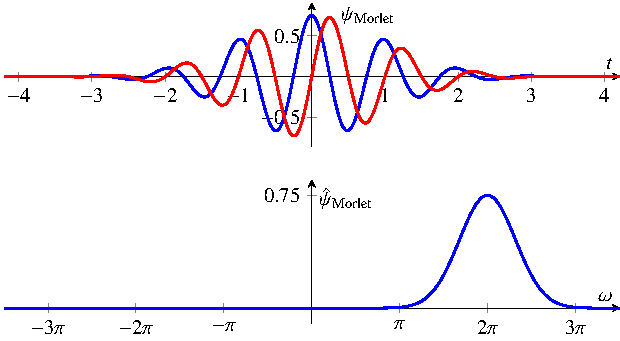
\includegraphics{papers/complex/images/morlet.pdf}
	\caption{Real- (blau) und Imaginärteil (rot) des Morlet-Wavelet für $\sigma = 2\pi$ \label{complex:morlet}}
\end{figure}

\begin{figure}
	\centering
	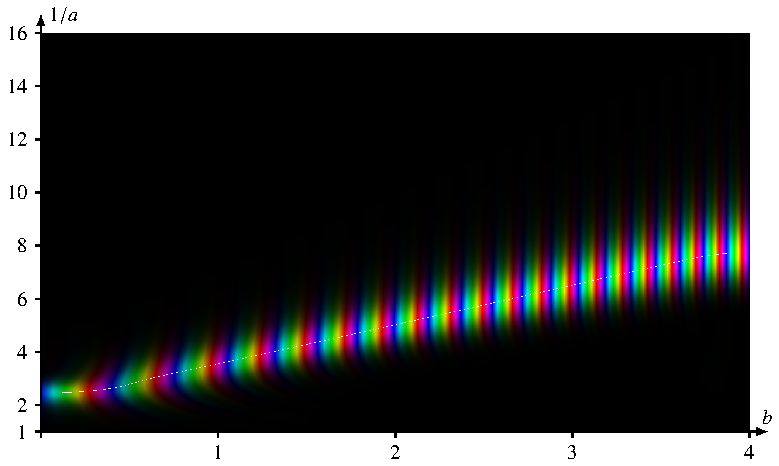
\includegraphics{papers/complex/images/chirp_morlet.pdf}
	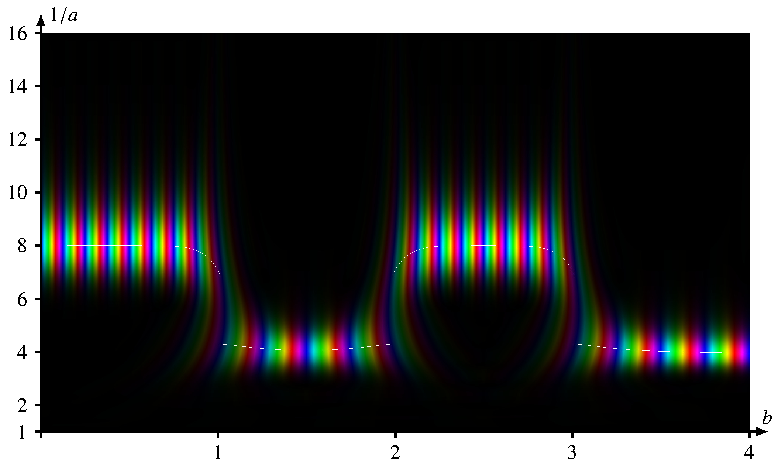
\includegraphics{papers/complex/images/square_morlet.pdf}
	\caption{Farb-codierte Wavelet-Transformationen der beiden Beispielsignale mit dem Morlet-Wavelet.}
	\label{complex:morlet-ex}
\end{figure}
